\chapter{Anexo A}

El Anexo A recoge y explica los procesos de instalación y configuración de los diferentes sistemas operativos, programas y herramientas necesarios para la implementación del proyecto.

% Configuración de la visualización del código SW
\lstset{backgroundcolor=\color{verde_p}, language=bash, breaklines=true, basicstyle=\footnotesize, xleftmargin=25pt, framesep=8pt, numbersep=15pt}


\section{Instalación de Raspbian OS}\label{anexo:raspbian}

Raspbian es un sistema operativo orientado a Raspberry Pi por lo que existe multitud de documentación complementaria en la web oficial\cite{Raspberry:2019}

Antes de comenzar a instalar el sistema operativo en una tarjeta microSD, se debe comprobar que ésta reúne los requisitos para ser usada en esta aplicación. Uno de estos requisitos es que la capacidad de la tarjeta sea superior a 8GB. Sin embargo, el uso de tarjetas de un tamaño superior a 32GB hace que sea necesario formatear la tarjeta antes de instalar el sistema operativo. Esto es debido a que el formato de serie (exFAT) no es compatible con el bootloader de Raspberry Pi, por lo que se deberá aplicar el formato FAT16 o FAT32 previamente.

Las instrucciones están pensadas teniendo en cuenta que se posee un ordenador con sistema operativo Windows.

\begin{enumerate}
\item \textbf{Descargar el sistema operativo}

Se puede descargar la imagen desde la web de descargas de Raspberry Pi\footnote{\url{https://www.raspberrypi.org/downloads/raspbian/}}

\begin{figure}[tb]
\centering
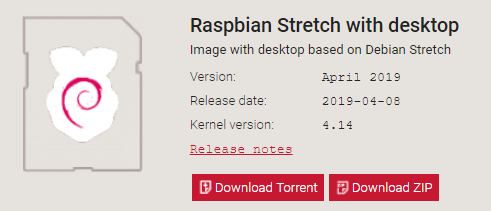
\includegraphics[width=0.5\textwidth]{figuras/RaspbianDwIcon.png}
\caption{Descarga de Raspbian Stretch}
\label{fig:descargaRaspbian}
\end{figure}

\item \textbf{Descargar e instalar Etcher}

Se precisa de una herramienta de escritura de imágenes y Etcher es la solución más sencilla para la mayoría de usuarios. Permite la escritura de la imagen sin la necesidad de extraer el archivo zip. 


\item \textbf{Escribir la imagen a una microSD}

Seleccionar el archivo de la imagen  la SD de destino es suficiente para flashear la imagen.

\item Una vez acabado el proceso de descompresión, la instalación debería estar completada. Introduciendo la tarjeta micro SD en su correspondiente posición en la Raspberry Pi, ésta acederá a Raspbian para arrancar el sistema.

\item Para comprobar la version del SO instalado, se puede hacer uso del comando \textit{lsb-release}

\begin{lstlisting}[frame=single, label=command:lsb]
lsb_release -a
\end{lstlisting}

\begin{figure}[tb]
\centering
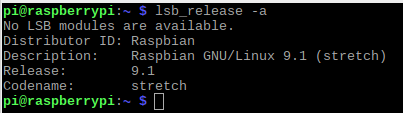
\includegraphics[width=0.5\textwidth]{figuras/RaspbianVersion.png}
\caption{Versión de Raspbian}
\label{fig:versionRaspbian}
\end{figure}

\end{enumerate}


\section{Instalación MQTT en Raspbian OS}\label{anexo:mqtt}

Mosquitto (broker de MQTT) se instala de igual manera que cualquier otra aplicación, haciendo uso de los repositorios.

En primer lugar, se actualizan los repositorios.

\begin{lstlisting}[frame=single, label=command:installmqtt1]
sudo apt-get update
\end{lstlisting}

Posteriormente, se instala Mosquitto.

\begin{lstlisting}[frame=single, label=command:installmqtt2]
sudo apt-get install mosquitto
\end{lstlisting}

Si todo va bien, al terminar el proceso, MQTT debería estar instalado.

Para probar la instalación, se pueden usar clientes de MQTT para enviar y recibir información a través un topic de prueba. Estos clientes son, por ejemplo, \textit{IoT MQTT Dashboard} en Android o \textit{MQTT.fx} en Windows.

\section{Edición y compilación de scripts en Raspbian OS}



\chapter{Anexo B}

En el Anexo B se sitúan los desarrollos software íntegros que forman parte del proyecto.

\section{Código SendAT.py}

\section{Código SendAPI.py}

\section{Código Receive.py}


\chapter{Anexo C}

El Anexo C recoge la documentación de interés de distintos componentes del proyecto

\section{Datasheet XBee Shield}